\chapter{Methodology} \label{method}
Evaluating new memory technologies without having physical access to them can be done by simulating their designs. There is always a measure of uncertainty and error when performing simulations, but it still gives a reasonable estimation of what to expect from the real hardware. Some argue that, e.g., cycle accurate simulators might not be the best approach in system evaluation \cite{weaver2008cycle}, but in this study all memories will be evaluated  using the same methodology with the same level of uncertainty. Thus the relationship between their performance should remain relevant. 
\bigskip

HMC is primarily meant to be put on the same substrate as a processor, but using several cubes in a chain topology is likely not a realistic approach. Although it would be supported by the HMC specification, it would be a hard, expensive and underperforming architecture to create and use. Having multiple network hops will inherently add latency and after a certain number of hops subsequent memory devices should arguably be regarded as far-memory, as opposed to being near-memory. With a setup consisting of memory with different access times, the system is a Non-uniform Memory Access (NUMA) system and an OS should place memory allocations as close as possible. The system could also use a simpler prefetching scheme in order to hide latency for sequential access, but that would also increase network load and possibly contention. In order to simplify this, we take a naive approach and regard all cubes as near-memory and we will only allocate memory on one device at a time. This will keep the results focused on impact of increasing number of hops rather than allocation schemes.
\bigskip

First in this chapter the simulation software for microarchitectures and memory technology is described. Next, a number of benchmark applications that will be run in the simulators are selected. Finally, the process of running applications and gathering results is defined.

%%%%%%%%%%%%%%%%%%%%%%%%%%%%%%  Simulators  %%%%%%%%%%%%%%%%%%%%%%%%%%%%%%

\section{Simulators}
For simulation of the memory network, two simulators were used: Structural Simulation Toolkit (SST) \cite{rodrigues2011structural} and HMCSim \cite{6969550}. The former was used for accurate microarchitecture simulation, while the latter was used to simulate the HMC memory. There were not many simulators for HMC available when this project started, which led to the use of HMCSim. This simulator in turn was already integrated with SST and this significantly lowered the amount of development needed to start. There has since come up other alternative HMC simulators \cite{7544479, Yang:2018:HCH:3240302.3240319} and there has also been created similar tools to accommodate multiple memory cubes in a network setup \cite{Siegl:2017:BAF:3132402.3132403}. Furthermore, the use of an HMC simulator with network support, as opposed to using a DRAM simulator with adjusted latencies, is justified by its detailed modelling of packet routing. The additional memory cubes in a network will ensure that memory requests are handled realistically with respect to packet handling, instead of naively increasing the link latency. To this end, the flexibility and extensibility of both HMCSim and SST has enabled a good basis for this kind of evaluation.
\bigskip

\subsection{SST}
SST is an architectural simulator which supports execution of x86 binaries towards different memory back-ends \cite{rodrigues2011structural}. It uses a modular front-end back-end framework, where each part can be replaced independently to model different architectural configurations. This modularity and the simulator's parallel simulation environment is enabled by the use of Message Passing Interface (MPI). This makes all communications event-based, and events are tagged with a delivery time. These events are only sent when needed and no real processing time is unnecessarily spent on future events \cite{11.1093/comjnl/bxr069}. Communication within the simulator uses a network model for routing information between components, which enables arbitrary architectural topologies. In addition, the router model can take network usage and congestion into account and monitor where and how often it occurs as well as if it caused any additional latencies.
\bigskip

Inside SST there are multiple ways of executing applications, where they are simulated in different ways. One way is to, on beforehand, run the application and save a memory trace of what the program did and then replay that inside the simulator using, e.g., \emph{Prospero}. This has the benefit of faster runtimes inside the simulator, while it will take some time and space to generate and store the memory trace. Another way is to run the application directly in the simulator using dynamic instrumentation of the programs' operations, which would be performed in the SST component \emph{Ariel}. Ariel, in turn, relies on Intel PIN Tool for running x86 binaries \cite{Luk:2005:PBC:1065010.1065034}. This has the major advantage that mostly any precompiled application can be run immediately through the simulator while also being faster than cycle-accurate models \cite{hammond2018structural}. It also supports thread interaction, but can on the other hand produce results that are not reproducible. Being an easy way to test memory systems, and providing a good trade-off between run-time and preparation time, it became our choice of processor model. It should be noted that SST is stuck on using PIN 2, whereas version 3 has been available for a few years. This is because the new version changes a few fundamental things in its operation, on which SST relies. Despite a collective effort to get support for PIN 3, it would require a major rewrite of the whole component -- which was outside the scope of this work.
\bigskip

The simulator's memory component is called \emph{memHierarchy} and encapsulates both memory controllers, interfaces and technologies. It is designed to be flexible and to easily incorporate new designs without changing too much in the existing logic. The component is also responsible for setting up and handling caches, coherence policies and buses. Additionally, inside memHierarchy is a memory controller which in turn is more appropriately named MemBackendConvertor. Here the conversion of application/CPU memory requests into memory backend specific requests are made. Furthermore, the backend is either a built-in memory model or an interface for an external tool, such as DRAMSim2 or the aforementioned HMCSim. All memory backends are written specifically for any external memory simulator, and HMCSim uses its own as well. In addition, it is also possible to use multiple backends simultaneously to enable further exploration of hybrid memory types.
\bigskip

With integration of HMCSim already present in the simulator, there were few changes needed in order to get a working simulation environment. While it was previously possible to configure multiple HMC devices in SST, it has not had any effect. As such, apart from the need to add support for multiple devices in HMCSim, there also needed to be some adaption to SST. Furthermore, there was no way to address more than one cube from SST and allocations would only have been done to the first device in the topology. Therefore, SST's memory access behaviour needed to be rewritten and after that it was possible to address all memory devices using unique identifiers. In addition, an attempt was made to spread out data across multiple nodes by allocating data on devices at random virtual addresses. The idea was that since HMC used a closed page policy, it would not matter where data was allocated, but it was determined that it would not be viable from a simulation perspective and could end up taking very long to run. In the end, only one memory unit will be used for data allocation per simulation.
\bigskip

Because of a limitation in HMCSim, communication to the network is only done using half of the configured links. This was different from the original behaviour, where all links could be used when having a single HMC device. While data is still being sent in parallel in all of the available links, if one link's queue gets full requests will be passed to another link. Moreover, it should remain theoretically possible to add a processor anywhere in this network, but there has been no validation whether SST's coherence mechanisms would still work when the HMC network is used in combination with SST's own. 
\bigskip

A crucial functionality SST lacked was to start simulating the program execution after a set number of instructions. To stop simulation after a number of instructions was supported from the start, but to start PIN instrumentation after a certain instruction count was not. Originally, SST required the application to call a specific function or the simulation had to trace the application from start. In order to speed up and get more relevant simulations, this support was added. In addition, instructions executed before tracing was started were run with little overhead and at relatively high speed.
\bigskip

In summary, the changes made to SST include:
\begin{itemize}
  \item Support for addressing more than one memory cube.
  \item Communication done over half of the configured links.
  \item Start instrumentation after a fix instruction count.
\end{itemize}
\bigskip

Lastly, one advantage of using SST when exploring on-chip networks is that arbitrary topologies of compute and memory nodes based on real products can be used. There have, however, been no effort made to match any existing products. As such, memory sizes, latencies and other configurations likely do not correspond to any real device since much of that information is proprietary. The CPU configuration is kept as simple as possible while remaining relatively realistic.

\subsection{HMCSim} \label{HMC-Sim}
HMCSim is, much unlike many other memory simulators available, primarily built with multidimensional memories in mind. This three dimensional approach enables a unique parallel access to banks, which is not accounted for in current memory simulation environments \cite{6969550}. Furthermore, because of HMC's tightly coupled logic die at the base of the memory stack, few other simulators can correctly mimic this integrated memory controller and parallel access scheme. HMCSim implements the HMC specification and enables simulation of HMC devices without physical access to one. It can either function alone from a memory trace or together with an architectural simulator sending memory requests from a running application. The first version of HMCSim implemented the initial versions of HMC, i.e., 1.0 and 1.1, whereas version two featured the additions made to specification 2.0 and 2.1. The latest and current version added support for power estimates.
\bigskip

HMCSim is designed to support all sorts of network topologies, both in the HMC logic layer and with multiple cubes. The user can set up how deep the queues for both the crossbar switch and the vault controller should be as well as measure latencies in clock cycles whenever packets are being delayed in queues. Furthermore, if, e.g., a write operation is sent with an address that is not physically closest to any of the vaults of the link the request happens to be sent through, the added latency of having to switch the packet through the crossbar switch to another vault is accounted for. While there is support for adding more devices and it is \emph{supported} to have them in a chain, the main functionality for adding more devices is connecting them in parallel to the host. This would be analogous to having a multiple memories connected over individual channels. In addition, the simulator supports different clock domains, and thus asynchronous operation, between host and memory devices so that memories, CPUs and SERDES links can use different frequencies. Furthermore, between version one and two, of both the HMC specification and the simulator, there were a few features added, such as support the new 256 byte read and write operations as well as Custom Memory Commands (CMC). One pre-made CMC is an atomic memory operation, where the base logic layer handles the atomicity and performs a read-modify-write by itself on its local memory stack \cite{7529923}. This does require application or compiler awareness, however, and as such is not used for our non-optimised programs.
\bigskip

HMCSim was already integrated as a memory backend in SST and the work to allow communication between a CPU model and the memory simulator was already done \cite{voskuilen2018sst}. The HMCSim integration utilises custom opcodes from SST to send commands to the memory, which also corresponds to how a HMC would work in a real application. While HMCSim has supported configurations of multiple devices, they could not communicate with one another. There was an awareness of other devices, but requests that were destined for another device were turned into zombie requests. The first addition to HMCSim was to support forwarding and routing of packets. The implementation is simple, building on what was already present, and seeks primarily to support this specific use case. A communication path was setup between devices that were linked together, and half of the available links were used to forward memory operations to the next device in line, as can be seen in \ref{HMCSim-network}. This leaves the last cube in the chain not fully utilising its links, and could be a place to add another host in the network without any additional loss of bandwidth. This approach was taken because of a technical limitation in HMCSim, where requests and following responses need to be sent over the same link. Furthermore, this effectively means that we have halved the available bandwidth compared to only connecting to one device. Since HMC specification is not very strict on how communication is done within a network this is still an acceptable solution.
\bigskip

\begin{figure}[!ht]
\centering
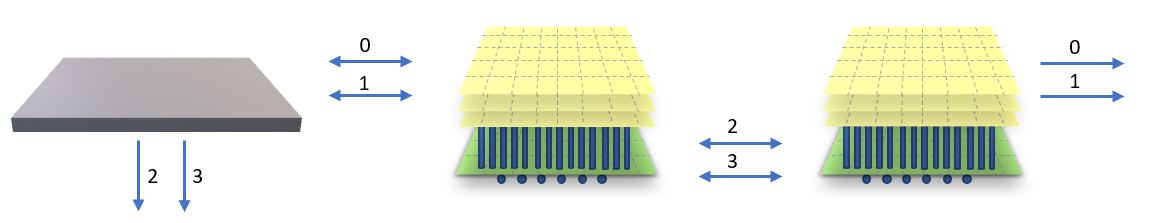
\includegraphics[width=0.75\linewidth]{figure/HMCSim-network.png}
\caption{The connections made between host and devices, as well as between devices. Note that request/response need to happen on the same link, hence the zig-zag appearance.}
\label{HMCSim-network}
\end{figure}

With support for inter-memory communication, there needed to be a topology set up as well. Furthermore, since there was no previous implementation for HMC networks in use, this was written from scratch. The basic topology interface created only allows for devices to be connected in chains and supports setting number of devices available. This is to show the worst case scenarios, and how multiple hops in a network will affect performance. Possible extensions to this implementation would be to allow for more topologies, or, more importantly, a way to easily create custom topologies. As mentioned earlier, the new implementation is not very flexible in its way of creating new topologies, as it works by manually designing link connections between devices in order to get a functioning network. While possible, it was not further explored and we considered that it would be enough to only measure worst-case scenarios.
\bigskip

To summarise, the following additions to HMCSim was introduced:
\begin{itemize}
  \item Network routing support between cubes.
  \item Using half of the configured links for communication.
  \item Rudimentary support for creating a topology.
\end{itemize}
\bigskip

In order to measure system latencies, the results obtained by Gokhale et al were interpreted as 93 ns with our setup \cite{10.1145/2833179.2833184}. Since we use a memory clock of 1 GHz this becomes 93 clock cycles of waiting. This is set as the base latency when accessing data in a DRAM array. All links are set to have a latency of 9 ns, where the high speed SERDES interface, switching time is taken into account. In addition to these latencies, there is also the routing of request and response data from each link to the corresponding vault where data is stored. A simple round robin scheme is used to access each available link from the host in order to distribute load as evenly as possible. It should be noted that no regard to the feasibility of having this many HMC devices on the same substrate is taken into account; quite possibly would only a subset of all configured memory cubes use the 9 ns latency, while devices farthest away would use an off-chip bus with a higher latency. For simplicity, all links are considered equal.

%%%%%%%%%%%%%%%%%%%%%%%%%%%%%%  Benchmarks  %%%%%%%%%%%%%%%%%%%%%%%%%%%%%%

\section{Benchmarks} \label{method-benches}
In order to evaluate performance of the system, a number of benchmarks from the SPEC CPU2006 was run \cite{henning2006spec}. Due to the amount of time it takes to simulate these different configurations, a few applications were selected based on their memory intensity. Prakash et al. did a performance characterization for the different benchmarks in SPEC, and determined that: \emph{mcf}, \emph{soplex}, \emph{lbm} and \emph{omnetpp} were among the ones with the most LLC misses, which means that they used the main memory the most \cite{prakash2008performance}. Similar studies have been made, which mostly come to the same conclusion regarding memory-bound applications \cite{4664856, 4086140, bird2007performance}. In addition, in order to test how a CPU-bound application reacts to the added memory latency, we also included \emph{namd} to the list. These five benchmarks should give us a good view of how different kinds of workloads behave in this setting. 
\bigskip

While applications should stress main memory in order to test a worst-case scenario, having diverse memory access patterns between the applications was equally important. With data being sent through both an external and internal memory network, the access pattern could impact how the application performs. A normal DRAM, with an open-page policy, can provide lower latency for accesses to different words in the same row, while accessing different rows in the same bank has higher latency \cite{10.1145/342001.339668}. Accessing consecutive data with a constant stride in order to exploit this lower latency is denoted as \emph{stream memory access}. This kind of access caches poorly and puts an additional strain on the main memory. The five applications chosen display quite different access behaviours in this regard, which further confirms the choice of benchmark applications \cite{10.1145/3307650.3322229, song2018experiments}.

%%%%%%%%%%%%%%%%%%%%%%%%%%%%%%%  Measurments  %%%%%%%%%%%%%%%%%%%%%%%%%%%%%%%

\section{Measurement approach}
Latency was only measured in HMCSim and any latency SST might introduce was disregarded. Furthermore, this made it easier to gather results, but did, on the other hand, make it impossible to see how long time it took for the execution to actually process the data. From HMCSim, we measured how often different latencies occurred and counted the average latency. The average latency was used to compare system configurations, while the distribution of access times gave us an idea of contention in the links and queues. We first performed a test run for a single HMC in order to establish application latency behaviour and sensitivity. Then we ran the same benchmarks using three, five and seven devices to determine how application performance maps towards latency. In addition, data was always allocated on the last device in the chain in order to maximise the number of hops, while minimising potential overhead with having more devices active in the simulator than is being used. Moreover, in order to avoid having to run entire applications we use a naive approach to limiting simulation time where the first one billion instructions are skipped, i.e. not simulated, and the instrumentation is limited to one billion instructions. Skipping the first one billion instructions will with a large likelihood ensure that the setting up of the application is not counted in the simulation, which in turn focuses the instrumentation time on the core algorithm and its memory access pattern. In addition, cache warm-up is set to one hundred million instructions. While this naive approach is not ideal, the alternatives required too much additional work to use. One method could have been SimPoint \cite{hamerly2005simpoint}, or rather PinPoint \cite{pinplay2010patil}, which is a version of SimPoints based on the workings of PIN. PinPoints could have been possible to use since PIN is already featured in the Ariel CPU model used in SST, but the replay of the so called Pinballs required changes far greater than what was in the scope for this thesis.
\bigskip

While a chain topology might not be viable approach for a real system, it enables us to focus on the worst-case scenario and the impact of the use of a network. As the allocations are done on the most distant device, all requests will have to propagate through the network. While this network is simulated, it does consist of multiple devices which all will handle and route the request to its destination. This means that all interaction in the network will be as close to a real system as possible. In contrast, by using a single memory device and increase the latency for every test, we would instead only see the effects of latency as opposed to view network impact.
\bigskip

The simulations were run on a by Chalmers provided compute cluster and took weeks, sometimes months, to complete. This cluster luckily used an older version of Ubuntu with a relatively old kernel, and since PIN 2 depends on older kernel functionality it meant it could be run without a hitch. In addition, in order to support the old ABI used with some of its binaries while having full support for C++11, GCC 4.9.4 had to be used, specifically. The setup and source code changes made to both simulators will be made public after publication\footnote{Here: https://github.com/yarcod}. 
\bigskip

The simulations were run with multiple configurations, where every application was configured to be run with either two or four links between each device, enabling between one and seven memory cubes. The reason for testing both two and four links is to see whether the increased bandwidth, and in this case amount of parallelism, would significantly impact latency or performance. Note that while HMC supports four and eight links in the specification, we can only use half of them from the host as the other half is used to interconnect the rest of the network, as explained in \ref{HMC-Sim}. Time of flight is measured from the CPU's point of view, i.e., from when it was first sent from the host to when the response arrived back. Execution time is measured during the time the application is traced in the simulator and is used to measure performance impact.
\bigskip